\chapter{Algoritmo de Grover}
%El algoritmo de Grover es un AC que encuentra con alta probabilidad la entrada única de una función de caja negra que produce un valor particular de salida, usando tan sólo $O(\sqrt{N})$ evaluaciones de la función, donde $N$ es el tamaño del dominio de la función. El análogo clásico de este algoritmo requiere $O(N)$ evaluaciones de la función, pues, el elemento correcto podría ser el $N$-ésimo en ser evaluado y se deben evaluar uno por uno. La aplicación directa de este algoritmo es como algoritmo de búsqueda en una base de datos. Sin embargo, su aplicación más eficiente es como subrutina en diversos procesos de optimización.

El algoritmo de Grover es un AC que realiza una búsqueda en una secuencia no ordenada de datos con $N=2^n$ entradas. Clásicamente esta búsqueda tendría un orden de complejidad de $O(N)$, pues, como los datos no están ordenados, la cantidad promedio de evaluaciones que se deben realizar crece linealmente con la cantidad de entradas. En el caso del algoritmo de Grover, la complejidad de la búsqueda es de $O(\sqrt{N})$, pues se requieren aproximadamente $\frac{\pi\sqrt{N}}{4}$ iteraciones para hallar la entrada deseada. En cuanto a la cantidad de qubits requeridos, se necesitan $O(\log_2 N)$ qubits, pues se debe realizar un estado superpuesto donde cada componente de la superposición represente una entrada de la secuencia de datos.

Supongamos que la secuencia de datos no ordenada tiene la siguiente función asociada:

\begin{equation}
    f(x) =
    \begin{cases}
        1 & \text{si } x = \omega \\
        0 & \text{si } x \neq \omega
    \end{cases}
\end{equation}

Donde $\omega$ es el dato que se desea encontrar. Esta función devuelve 1 si se evalua la entrada que almacena el dato deseado y 0 en cualquier otro caso.

El algoritmo de Grover se basa en la disponibilidad de un operador cuántico, llamado \textit{oráculo}, tal que se introduzca un fase global de $\pi$ si $f(x_0)=1$ y deje el estado del sistema intacto si $f(x_0)=0$. Es decir, el oráculo realiza una reflexión alrededor de $\ket{\omega}$.

\begin{equation}
    U_\omega \ket{x} = (-1)^{f(x)} \ket{x} =
    \begin{cases}
        \ket{x} & \text{si } x \neq \omega \\
        - \ket{x} & \text{si } x = \omega
    \end{cases}
\end{equation}

\begin{equation}
U_\omega = \mathds{1} - 2 \ketbra{\omega}{\omega}
\end{equation}

Además de éste, se necesita otro operador de reflexión, $U_s$, el cual realiza una reflexión alrededor del estado de superposición uniforme $\ket{s} = \frac{1}{\sqrt{N}} \sum\limits_{x=0}^{N-1} \ket{x}$. Así, por el hecho de la geometría plana elemental de que el producto de dos reflexiones es una rotación, se logra aproximar el estado del sistema al estado asociado a la entrada deseada.

\begin{equation}
U_s = 2 \ketbra{s}{s} - \mathds{1}
\end{equation}

Veamos lo que sucede al aplicar esta secuencia de rotaciones sobre el estado $\ket{s}$:

\begin{multline}
    U_\omega \ket{s}
    = (\mathds{1} - 2 \ketbra{\omega}{\omega}) \ket{s}
    = \ket{s} - 2 \ketbra{\omega}{\omega} \ket{s} \\
    = \ket{s} - \frac{2}{\sqrt{N}} \ketbra{\omega}{\omega} \sum\limits_{x=0}^{N-1} \ket{x}
    = \ket{s} - \frac{2}{\sqrt{N}} \ket{\omega}
\end{multline}

\begin{multline}
    U_s (\ket{s} - \frac{2}{\sqrt{N}} \ket{\omega})
    = (2 \ketbra{s}{s} - \mathds{1}) (\ket{s} - \frac{2}{\sqrt{N}} \ket{\omega}) \\
    = 2 (\ket{s} - \frac{4}{N} \ket{s}) - (\ket{s} - \frac{2}{\sqrt{N}} \ket{\omega})
    = \ket{s} - \frac{4}{N} \ket{s} + \frac{2}{\sqrt{N}} \ket{\omega} \\
    = \frac{N-4}{N} \ket{s} + \frac{2}{\sqrt{N}} \ket{\omega}
\end{multline}

Ahora veamos lo que sucede al aplicar esta secuencia de rotaciones sobre el estado $\ket{\omega}$:

\begin{equation}
    U_\omega \ket{\omega}
    = (\mathds{1} - 2 \ketbra{\omega}{\omega} \ket{\omega}
    = \ket{\omega} - 2 \ket{\omega}
    = - \ket{\omega}
\end{equation}

\begin{equation}
    U_s (-\ket{\omega})
    = (2 \ketbra{s}{s} - \mathds{1}) (-\ket{\omega})
    = -\frac{2}{\sqrt{N}} \ket{s} + \ket{\omega}
\end{equation}

Se observa que al aplicar $U_s U_\omega$ sobre $\ket{s}$, se amplifica la componente de $\ket{\omega}$ en la superposición de $\frac{1}{\sqrt{N}}$ a $\frac{3N-4}{N \sqrt{N}}$. Es decir que la probabilidad de medir el valor deseado crece de $\frac{1}{N}$ a $9 (1-\frac{4}{3N}) \frac{1}{N}$.

\begin{equation}
    \bra{\omega} U_s U_\omega \ket{s}
    = \frac{N-4}{N} \frac{1}{\sqrt{N}} + \frac{2}{\sqrt{N}}
    = \frac{3N-4}{N \sqrt{N}}
\end{equation}

\begin{equation}
    p(\omega) = \abs{\bra{\omega} U_s U_\omega \ket{s}}^2
    = \frac{(3N-4)^2}{N^3}
    = 9 (1-\frac{4}{3N}) \frac{1}{N}
    \label{eq:prob1step}
\end{equation}

Por otro lado, se observa que al aplicar $U_s U_\omega$ sobre $\ket{\omega}$, aparece una componente de $\ket{s}$, así que en ese caso, la probabilidad de medir el valor deseado disminuye. Por lo que debe existir una cantidad de iteraciones $k_{max}$ tras las cuales se alcanza la probabilidad máxima de medir $\ket{\omega}$, partiendo de $\ket{s}$ y a partir de donde esta probabilidad empieza a disminuir.

De esta manera, el algoritmo de Grover consiste en aplicar $k_{max}$ veces $U_s U_\omega$, partiendo del estado $\ket{s}$, es decir rotar este estado hasta que se aproxime lo más posible a $\ket{\omega}$.

\begin{figure}[H]
\[ \Qcircuit @C=1.4em @R=1.8em {
\lstick{\ket{0}} & {/^n} \qw & \gate{H^{\otimes n}} & \gate{U_{\omega}} & \gate{U_s} & \meter & \cw \\
& & & \rstick{\hspace{-13pt} k_{max} \text{ veces}}
\gategroup{1}{4}{1}{5}{1.5em}{_\}}
} \]
\caption{Circuito del algoritmo de Grover, $k_{max}$ desconocido.}
\end{figure}

Para hallar $k_{max}$, veamos el ángulo que se rota con cada aplicación de $U_s U_\omega$. Primero definamos el estado $\ket{s^\prime}$ como la superposición uniforme de todos los estados de la base computacional excepto $\ket{\omega}$, es decir:

\begin{equation}
    \ket{s^\prime} = \frac{1}{N-1} \sum\limits_{x \neq \omega} \ket{x}
               = \frac{\sqrt{N}}{\sqrt{N-1}}\ket{s} - \frac{1}{\sqrt{N-1}} \ket{\omega}
\end{equation}

Los estados $\ket{s^\prime}$ y $\ket{\omega}$ son ortonormales, $\braket{s^\prime}{\omega} = 0$, por lo que generan un espacio bidimensional de Hilbert. Este espacio contiene a $\ket{s}$, pues:

\begin{equation}
    \ket{s} = \frac{\sqrt{N-1}}{\sqrt{N}}\ket{s^\prime} + \frac{1}{\sqrt{N}}\ket{\omega}
\end{equation}

Además, se ha visto que $U_s U_\omega \ket{s}$ y $U_s U_\omega \ket{\omega}$ se escriben en función de sólo $\ket{s}$ y $\ket{\omega}$. Así que podemos inducir que $(U_s U_\omega)^k \ket{s}$ pertenece al espacio generado por $\{\ket{s^\prime}, \ket{\omega}\}$, donde $k \in \{0, 1, 2, ...\}$. Esto indica que este espacio contiene al plano en el que se realizan las rotaciones $U_s U_\omega$.

Ahora que conocemos una base del plano de rotación, podemos hayar el ángulo que se rota con cada aplicación de $U_s U_\omega$.

\begin{equation}
    U_\omega \ket{\psi}
    = (\mathds{1} - 2 \ketbra{\omega}{\omega}) (\alpha \ket{s^\prime} + \beta \ket{\omega})
    = \alpha \ket{s^\prime} - \beta \ket{\omega}
\end{equation}

\begin{multline}
    U_s (\alpha \ket{s^\prime} - \beta \ket{\omega})
    = (2 \ketbra{s}{s} - \mathds{1}) (\alpha \ket{s^\prime} - \beta \ket{\omega}) \\
    = \alpha \left(2 \frac{\sqrt{N-1}}{\sqrt{N}} \ket{s} - \ket{s^\prime}\right) - \beta \left(\frac{2}{\sqrt{N}} \ket{s} - \ket{\omega}\right) \\
    = \alpha \left((2\frac{N-1}{N} - 1) \ket{s^\prime} + 2\frac{\sqrt{N-1}}{N}\ket{\omega}\right)
    - \beta \left(\frac{2\sqrt{N-1}}{N}\ket{s^\prime} + (\frac{2}{N}-1)\ket{\omega}\right) \\
    = (\alpha \frac{N-2}{N} - \beta \frac{2\sqrt{N-1}}{N}) \ket{s^\prime}
    + (\alpha\ 2\frac{\sqrt{N-1}}{N} + \beta  \frac{N-2}{N}) \ket{\omega} \\
\end{multline}

De aquí se deduce que $\cos(\Delta\theta) = \frac{N-2}{N}$ y que $\sin(\Delta\theta) = 2\frac{\sqrt{N-1}}{N}$. De hecho, se comprueba que:

\begin{equation}
    \cos^2(\Delta\theta)+\sin^2(\Delta\theta)
    = \frac{(N-2)^2}{N^2} + 4\frac{N-1}{N^2}
    = \frac{N^2-4N+4}{N^2} + 4\frac{N-1}{N^2}
    = 1
\end{equation}

Ahora escribimos las componentes de $\ket{s}$ en función del ángulo inicial $\theta_0$:

\begin{align}
    \cos(\theta_0) &= \frac{\sqrt{N-1}}{\sqrt{N}} \\
    \sin(\theta_0) &= \frac{1}{\sqrt{N}}
    \label{eq:sinTheta0}
\end{align}

Finalmente, lo que se quiere es que:

\begin{equation}
    \theta_0 + k \Delta\theta \to \frac{\pi}{2}
\end{equation}

Es decir, que:

\begin{align}
    \cos^{-1}(\frac{\sqrt{N-1}}{\sqrt{N}}) + k\cos^{-1}(\frac{N-2}{N}) &\to \frac{\pi}{2} \\
    \sin^{-1}(\frac{1}{\sqrt{N}}) + k\sin^{-1}(2\frac{\sqrt{N-1}}{N}) &\to \frac{\pi}{2}
\end{align}

Si tomamos $N \gg 1$ en (4.12), tenemos que:

\begin{align}
    2k \frac{1}{\sqrt{N}} &\to \frac{\pi}{2} \\
    k_{max} &\approx \frac{\pi \sqrt{N}}{4}
\end{align}

\begin{figure}[H]
\centering 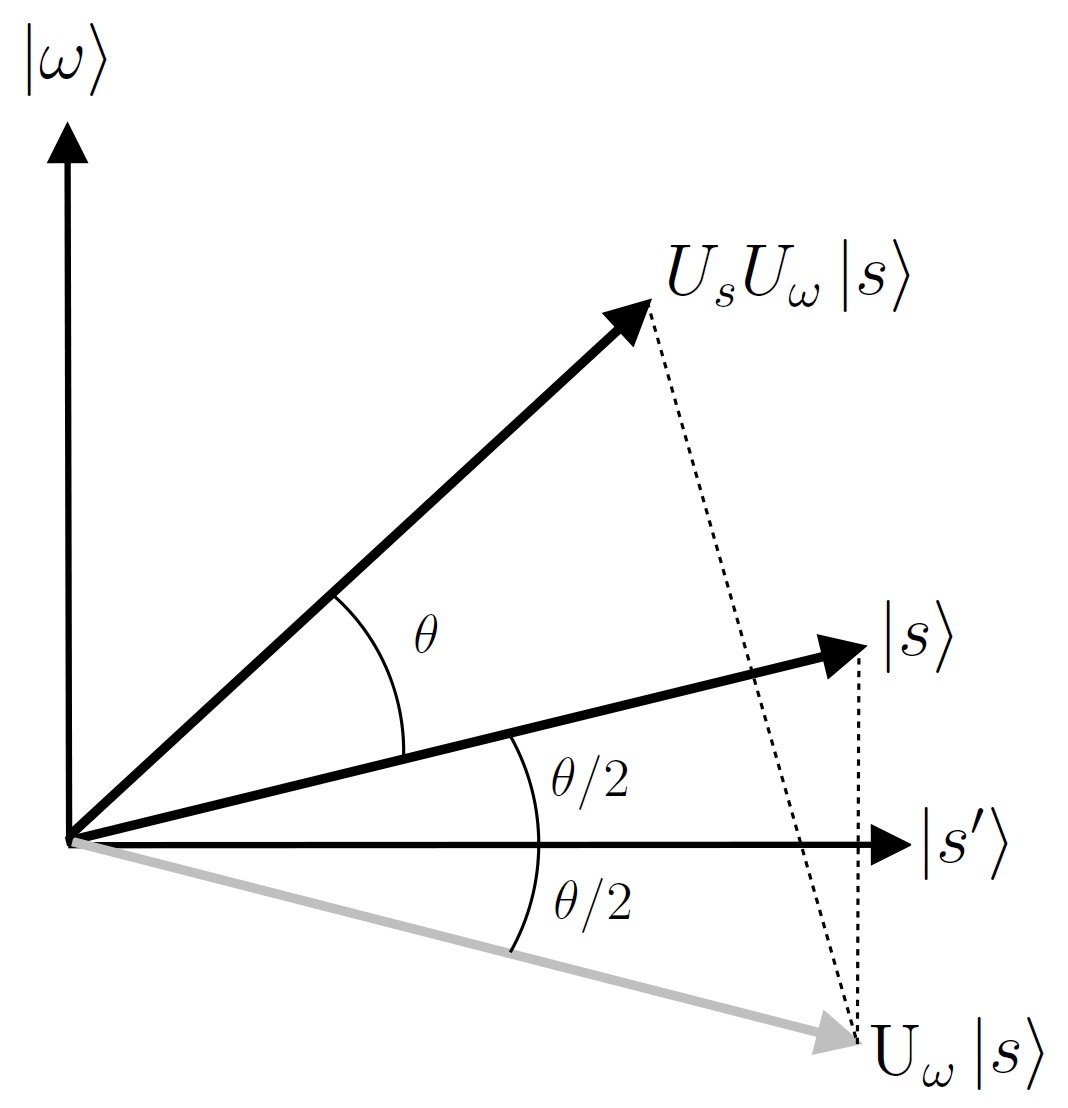
\includegraphics[width=0.3\linewidth]{img/grover_geometry.png}
\caption{Interpretación geométrica del operador difusión}
\end{figure}

\section{El algoritmo}

\begin{figure}[H]
\[ \Qcircuit @C=1.4em @R=1.8em {
\lstick{\ket{0}} & {/^n} \qw & \gate{H^{\otimes n}} & \gate{U_{\omega}} & \gate{U_s} & \meter & \cw \\
& & & \rstick{\hspace{-13pt} \lfloor\frac{\pi \sqrt{N}}{4}\rfloor \text{ veces}}
\gategroup{1}{4}{1}{5}{1.3em}{_\}}
} \]
\caption{Circuito del algoritmo de Grover.}
\end{figure}

\begin{enumerate}
    \item Preparar el estado fiducial.
    \item Aplicar la transformada de Walsh-Hadamard.
    \item Realizar la iteración de Grover $\lfloor \frac{\pi}{4} \sqrt{N} \rfloor$ veces.
    \begin{enumerate}
        \item Aplicar $U_{\omega}$.
        \item Aplicar $U_s$.
    \end{enumerate}
    \item Realizar la medida $\Omega$.
\end{enumerate}

\section{Variaciones y generalizaciones del algoritmo de Grover}

A continuación estudiaremos el algoritmo de amplificación de amplitud, el cual es una generalización del algoritmo de Grover para bases de datos con cualquier cantidad de estados objetivos, y el algoritmo de Grover en un paso, el cual es una variación del algoritmo de Grover en la que se mide en cada iteración.

\subsection{Algoritmo de amplificación de amplitud}

Esta generalización fue desarrollada independientemente por Brassar y H̨\o yer en 1997 [ref] y por Grover en 1998 [ref]. Con este algoritmo se pueden utilizar funciones oráculo que marquen 1 para más de una entrada de la base de datos en la cual se realizará la búsqueda. Entonces, sea $\mathcal{W}$ el conjunto de entradas a encontrar, tenemos la función oráculo:

\begin{equation}
    f(x) =
    \begin{cases}
        1 & \text{si } x \in \mathcal{W} \\
        0 & \text{si } x \not\in \mathcal{W}
    \end{cases}
\end{equation}

Ahora sea el proyector $\Pi_\mathcal{W}$ tal que proyecte los estados del espacio de Hilbert $\mathcal{H}$ asociado a la base de datos en el espacio de Hilbert generado por los estados objetivos $\mathcal{H}_\mathcal{W}$:

\begin{equation}
    \Pi_\mathcal{W} = \sum\limits_k \ketbra{\omega_k}{\omega_k}
\end{equation}

Donde los estados $\ket{\omega_k}$ son los estados asociados a las entradas de la base de datos pertenecientes a $\mathcal{W}$.

Sea el estado inicial:

\begin{equation}
    \ket{\psi} = \sin(\theta) \ket{\psi_1} + \cos(\theta) \ket{\psi_0}
\end{equation}

Donde $\ket{\psi_1} = \frac{\Pi_\mathcal{W} \ket{\psi}}{\sin(\theta)}$ y $\sin(\theta) = \bra{\psi} \Pi_\mathcal{W} \ket{\psi}$. De aquí podemos hallar que $\ket{\psi_0} = \frac{(\mathds{1} - \Pi_\mathcal{W}) \ket{\psi}}{\cos(\theta)}$ y que $\cos(\theta) = \bra{\psi} (\mathds{1} - \Pi_\mathcal{W}) \ket{\psi}$.

Ahora definamos los siguientes operadores de reflexión $U_\psi = (2 \ketbra{\psi}{\psi}$ y $ U_\mathcal{W} = \mathds{1})(\mathds{1} - 2 \Pi_\mathcal{W})$, estos son las generalizaciones de $U_s$ y $U_\omega$, del algoritmo de Grover, respectivamente. El producto de ellos, $U_\psi U_\mathcal{W}$ es un operador de rotación en el plano generado por $\ket{\psi_0}$ y $\ket{\psi_1}$, de la misma manera que $U_s U_\omega$ es un operador de rotación en el plano generado por $\ket{s^\prime}$ y $\ket{\omega}$. Ahora veamos el efecto de $U_\psi U_\mathcal{W}$ y el ángulo que rota este operador:

\begin{multline}
    U_\psi U_\mathcal{W} \ket{\psi} = (2 \ketbra{\psi}{\psi} - \mathds{1}) (\mathds{1} - 2 \Pi_\mathcal{W}) \ket{\psi} = (2 \ketbra{\psi}{\psi} - \mathds{1}) [(\mathds{1} - \Pi_\mathcal{W}) - \Pi_\mathcal{W}] \ket{\psi} \\
    = (2 \ketbra{\psi}{\psi} - \mathds{1}) (\cos(\theta) \ket{\psi_0} - \sin(\theta) \ket{\psi_1}) = (2 \ketbra{\psi}{\psi} - \mathds{1}) (\ket{\psi} - 2 \sin(\theta) \ket{\psi_1}) \\
    = \ket{\psi} + (- 4 \sin^2(\theta) \ket{\psi} + 2 \sin(\theta) \ket{\psi_1}) = (3 - 4 \sin^2(\theta)) \sin(\theta) \ket{\psi_1} + (1 - 4 \sin^2(\theta)) \cos(\theta) \ket{\psi_0} \\
    = \sin(3 \theta) \ket{\psi_1} + \cos(3 \theta) \ket{\psi_0}
    \label{eq:DTheta}
\end{multline}

Como se puede ver, el operador $U_\psi U_\mathcal{W}$ rota un ángulo de $2 \theta$. Por lo que si se aplica $k$ veces a $\ket{\psi}$, tendremos:

\begin{equation}
    (U_\psi U_\mathcal{W})^k \ket{\psi} = \sin( (2 k + 1) \theta) \ket{\psi_1} + \cos( (2 k + 1) \theta) \ket{\psi_0}
\end{equation}

De esta manera, el $k = k_max$ para el cual se obtiene la probabilidad máxima de medir un elemento de $\mathcal{H}_\mathcal{W}$, es decir, el $k$ que maximiza la amplitud de probabilidad de la componente $\ket{\psi_1}$ de $\ket{\psi}$, es $\lfloor \frac{\pi}{4 \theta} \rfloor$. Así:

\begin{multline}
    (U_\psi U_\mathcal{W})^{k_{max}} \ket{\psi} = \sin( (2 \lfloor \frac{\pi}{4 \theta} \rfloor + 1) \theta) \ket{\psi_1} + \cos( (2 \lfloor \frac{\pi}{4 \theta} \rfloor + 1) \theta) \ket{\psi_0} \\
    \approx \sin(\frac{\pi}{2}) \ket{\psi_1} + \cos(\frac{\pi}{2}) \ket{\psi_0} = \ket{\psi_1}
\end{multline}

Mientras menor sea $\theta$, más tenderá $(U_\psi U_\mathcal{W})^{k_{max}} \ket{\psi}$ a $\ket{\psi_1}$, pero mayor será $k_{max}$.

Como se puede ver, el algoritmo de amplificación de amplitud se puede utilizar como algoritmo de búsqueda con una cantidad arbitraria de estados objetivos y un estado inicial arbitrario, no sólo $\ket{s}$ como en el algoritmo de Grover. Sin embargo, este no es sólo un algoritmo de búsqueda, sino tambien un algoritmo de optimización. En este sentido, la amplificación de amplitud también se puede utilizar como subrutina para mejorar el resultado de otros algoritmos. Sea $U_\mathcal{A}$ el operador asociado a un algoritmo cuántico $\mathcal{A}$, entonces, tal que, partiendo del estado fiducial, retorne el estado $\ket{\psi}$. Es decir, $U_\mathcal{A} \ket{0} = \ket{\psi}$, entonces, podemos reescribir $U_\psi$ de la siguiente manera:

\begin{equation}
    U_\psi = (2 \ketbra{\psi} - \mathds{1}) = (2 U_\mathcal{A} \ketbra{0} U_\mathcal{A}^\dagger - \mathds{1}) = U_\mathcal{A} (2 \ketbra{0} - \mathds{1}) U_\mathcal{A}^\dagger = U_\mathcal{A} U_0 U_\mathcal{A}^\dagger
\end{equation}

De esta manera, a cualquier algoritmo, que actúe sobre un espacio de Hilbert $\mathcal{H}$ que se pueda descomponer un espacio de estados buenos $\mathcal{H}_\mathcal{W}$ y un espacio de estados malos $\mathcal{H} \setminus \mathcal{H}_\mathcal{W}$, se le puede aplicar la amplificación de amplitud para mejorar su resultado.

Ahora consideremos el caso en el que $U_\mathcal{A} = H^{\otimes n}$, es decir, el caso en el que $\ket{\psi} = \ket{s}$. Este seria el caso particular del algoritmo de amplificación de amplitud en el que se utiliza el mismo estado inicial del algoritmo de Grover.

\begin{align}
    \ket{\psi} &= \frac{1}{\sqrt{N}} \sum\limits_i \ket{i} = \frac{1}{\sqrt{N}} \sum\limits_{i \in \mathcal{W}} \ket{i} + \frac{1}{\sqrt{N}} \sum\limits_{j \not\in \mathcal{W}} \ket{j} \\
    \ket{\psi_1} &= \frac{1}{\sqrt{W}} \sum\limits_{i \in \mathcal{W}} \ket{i} \\
    \sin{\theta} &= \sqrt{\frac{W}{N}} \\
    \ket{\psi_0} &= \frac{1}{\sqrt{N-W}} \sum\limits_{j \not\in \mathcal{W}} \ket{j} \\
    \cos{\theta} &= \sqrt{\frac{N-W}{N}}
\end{align}

Si tomamos $N \gg W$, tendríamos que $\theta \approx \sqrt{\frac{W}{N}}$, entonces $k_{max} \approx \frac{\pi}{4} \sqrt{\frac{N}{W}}$. Es interesante notar que mientras más estados buenos haya, menos iteraciones se necesitan. Pero a cambio, para hallar todos esos estados buenos, se debe ejecutar el algoritmo más veces. En caso de que $\mathcal{W}$ sea de dimensión 1, se recuperaría exactamente el algoritmo de Grover.

\subsection{Algoritmo de Grover en un paso}

En [ref] Grover propone una manera alternativa para ejecutar su algoritmo. En lugar de realizar $O(\sqrt{N})$ iteraciones, propone realizar una sola iteración en $\Omega(\sqrt{N \log(N)})$ sistemas identicos simultáneamente. Partiendo de la ecuación \ref{eq:prob1step}, la probabilidad de medir cada uno de los estados, cuando N es grande, luego de aplicar una iteración del algoritmo de Grover es aproximadamente:

\begin{equation}
    p(x) \approx
    \begin{cases}
        \frac{9}{N} & \text{si } x = \omega \\
        \frac{1}{N} & \text{si } x \neq \omega
    \end{cases}
\end{equation}

Así que con $\eta$ sistemas se tendrá, en promedio $9 \eta/N \pm O(\sqrt{\eta/N})$ medidas del valor deseado y $\eta/N \pm O(\sqrt{\eta/N})$ medidas de cualquiera de cada uno de los otros estados. La idea es tener suficientes sistemas para poder elegir con seguridad el valor que más se repita como el valor deseado. Por el teorema del límite central, la probabilidad de que una variable particular se desvíe más de $\pm \gamma \sqrt{\eta/N}$ de su valor esperado es menor que $e^{- \Omega(\gamma^2)}$. De esta manera, si $\eta = \Omega(N \log(N))$, entonces, con una probabilidad cercana a 1, el valor deseado ocurrirá con mayor frecuencia que cualquiera de los otros $N-1$.

Este esquema también se puede aplicar al algoritmo de amplificación de amplitud, pero con una condición: Que la cantidad de estados marcados sea menor a $N/4$. Esto es porque no hay manera de diferenciar los $W$ estados deseados de los otros $N - W$. Entonces, si $W$ es cercano a $N/2$, resultará imposible identificar correctamente los estados deseados.

Es importante mencionar que aunque esta versión del algoritmo se pueda ejecutar con una sola iteración, resulta menos eficiente que el algoritmo de Grover tradicional. Esto es porque esas $\Omega(N \log(N))$ mediciones necesitarán ser procesadas para hallar los valores más frecuentes, lo cual tendrá una complejidad temporal del mismo orden $\Omega(N \log(N))$, la cual es mayor a la complejidad temporal $O(\sqrt{N}$ de la versión tradicional del algoritmo. De esta forma, la única verdadera ventaja de esta variacíón estaría en el caso en que se tengan sistemas con tiempos de vida tales que no permitan realizar las iteraciones necessarias para ejecutar la versión tradicional del algoritmo de Grover.

\subsection{Optimización del algoritmo de Grover}

En [ref] Garg y Pande proponen una optimización del algoritmo de Grover, mezclando el algoritmo de Grover tradicional y el algoritmo de Grover de un paso. La idea de ellos es ejecutar el algoritmo en múltiples sistemas idénticos, como en el algoritmo de un paso, pero realizar más de una iteración, como en el algoritmo tradicional. De esta manera, reducen la cantidad $\eta$ de sistemas necesarios y la cantidad $k$ de iteraciones necesarias. Ellos hayan que tomando $\eta = k$, entonces sólo se necestian $O(\sqrt[3]{N})$.

Partiendo de \ref{eq:sinTheta0} y \ref{eq:DTheta}, sabemos que en cada iteración de Grover, cuando $N$ es grande, se rota un ángulo de aproximadamente $2/\sqrt{N}$ y que el ángulo inicial es aproximadamente $1/\sqrt{N}$. Así que luego de $k$ iteraciones, se tendrá un ángulo de aproximadamente $(2k + 1)/\sqrt{N}$. Por lo tanto, la probabilidad de medir cada estado será:

\begin{equation}
    p(x) \approx
    \begin{cases}
        \frac{(2k + 1)^2}{N} & \text{si } x = \omega \\
        \frac{1}{N} & \text{si } x \neq \omega
    \end{cases}
\end{equation}

Si realizamos esto en $\eta$ sistemas idénticos, entonces, mediremos el valor deseado $\eta (2k + 1)^2 / N \pm O(\sqrt{\eta k^2/N})$ veces y cada otro estado $\eta / N \pm O(\sqrt{\eta k^2/N})$ veces. Si tomamos $\eta = k$, entonces, mediremos $\omega$ alrededor de $k (2k + 1)^2 / N \pm O(\sqrt{k^3/N})$ veces. Ahora, si tomamos $k$ en el orden de $O(\sqrt[3]{N})$, tendremos $\omega$ alrededor de $\sqrt[3]{N} ( 2 \sqrt[3]{N} + 1)^2 \pm O(1)$ veces. Como $N$ es grande, podemos hacer la aproximación $2 \sqrt[3]{N} + 1 \approx 2 \sqrt[3]{N}$ y entonces, tendremos $\omega$ alrededor de $4 \pm O(1)$ veces. Mientras que todos los otros valores ocurriran sólo $N^{-2/3} \pm O(1)$ veces cada uno. Así que, el estado medido con mayor frecuencia ha de ser, con seguridad, el estado deseado.

Finalmente, la parte cuántica de este algoritmo tiene una complejidad temporal de $O(\sqrt[3]{N})$ y el procesamiento posterior de las mediciones realizadas también tendrá una complejidad temporal de $O(\sqrt[3]{N}$, pues esta es la cantidad de datos a procesar. Por lo tanto, la complejidad total de este algoritmo es $O(\sqrt[3]{N}$, la cual es menor a $O(\sqrt{N})$ de la versión tradicional y a $\Omega(N \log(N))$ de la versión en un paso.

\section{Simulaciones}

Se realizaron simulaciones del algoritmo de Grover con $\ket{\omega} = \ket{0000}$, $\ket{\omega} = \ket{0110}$ y $\ket{\omega} = \ket{1111}$. También se realizon simulaciones del algoritmo de amplificación de amplitud con $\mathcal{W} = \{ \}$ y $\mathcal{W} = \{ \}$.

Un conjunto de las simulaciones se ha realizado en Wolfram Mathematica, implementando los operadores, es decir $U_{\omega}$, $U_\mathcal{W}$, $U_s$ y la transformada de Hadamard, directamente, de manera matricial, de acuerdo a las definiciones dadas anteriormente. Otro conjunto de las simulaciones ha realizado en Python, definiendo todos los operadores y transformaciones en base a sus construcciones circuitales, a partir de las compuertas nativas de los transmones, resolviendo la ecuación maestra del sistema al aplicar cada compuerta nativa. Al primer conjunto lo llamaremos simulaciones matemáticas, y al segundo, simulaciones circuitales. El código todas las simulaciones de este capítulo se encuentra en el apéndice \ref{ch:grovercod}.

En el caso de la simulaciones matemáticas, sólo se ha simulado el caso sin relajación. Por otro lado, en el caso de la simulaciones circuitales, se ha simulado el sistema tanto sin relajación, como con relajación. En el caso del sistema con relajación, se ha utilizado la ecuación maestra de Lindblad con los operadores de colapso $\sigma_{-_i}$ y tasa de relajación $\gamma = 25KHz$.

\subsection{Algoritmo de Grover}

Como el espacio de Hilbert del sistema en el que sea ejecutado el algoritmo es de 16 dimensiones, ya que es de cuatro qubits, se necesitan $\lfloor \frac{\pi \sqrt{16}}{4} \rfloor = 3$ iteraciones para tener la máxima probabilidad de medir el estado deseado. Sin embargo, la simulación se ha realizado con 7 iteraciones, para apreciar la naturaleza oscilatoria de este algoritmo. Recordemos que este algoritmo consiste en rotaciones en el espacio 2D generado por $\ket{\omega}$ y $\ket{s^\prime}$, es decir, que si se aplican más de 3 rotaciones, la probabilidad de éxito debería disminuir, hasta que el estado del sistema se alinee con $- \ket{s^\prime}$, volver a aumentar hasta llegar a $- \ket{\omega}$, disminuir hasta pasar por $\ket{s^\prime}$, pasar de nuevo por el estado inicial $\ket{s}$ y repetirse el ciclo. La hipotesis es que veremos aproximadamente un período de sinusoide muestreada, con alrededor de seis muestras por período, en la gráfica de la evolución de la probabilidad de medir $\ket{\omega}$, ya que si luego de tres iteraciones se llega al punto de probabilidad máxima, alrededor de la sexta iteración se debe llegar al punto de probabilidad mínima y en la séptima volvería a aumentar.

En la figura \ref{fig:groverlosslesscomp1111} se puede observar la gráfica de la evolución de la probabilidad de medir cada estado en cada iteración del algoritmo de Grover con $\ket{\omega} = \ket{1111}$. Como se puede observar, ambas figuras son bastante similares. La fidelidad entre los estados finales de ambas simulaciones es 0.999875. Además, se ha confirmado la hipotesis de que la evolución de la probabilidad de medir $\ket{1111}$ tiene forma sinusoidal.

\begin{figure}[H]
    \centering
    \begin{subfigure}[m]{0.49\textwidth}
        \centering
        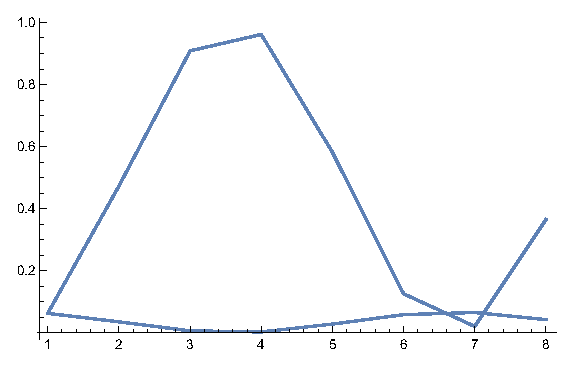
\includegraphics[width=0.9\linewidth]{img/Grover-2_gr1.eps}
        \caption{Wolfram Mathematica}
    \end{subfigure}
    \begin{subfigure}[m]{0.49\textwidth}
        \centering
        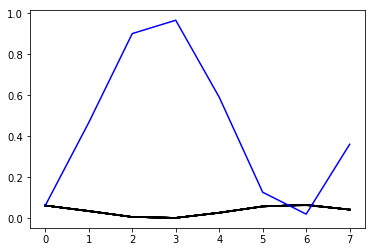
\includegraphics[width=0.9\linewidth]{img/groveralllossless.png}
        \caption{Python}
    \end{subfigure}
    \caption[Evolución de las probabilidades en el algoritmo de Grover sin relajación]{Evolución de las probabilidades en el algoritmo de Grover sin relajación}
    \label{fig:groverlosslesscomp1111}
\end{figure}

Ahora, compararemos los resultados de la simulación circuital con y sin relajación. Como se puede ver en la figura \ref{fig:groverlosscomp}, en el caso con relajación, los estados que no contienen el valor deseado dejan de tener todos la misma probabilidad. Los estados que involucran el estado base ganan probabilidad debido a la relajación de los qubits. La fidelidad entre los estados resultantes de los casos con y sin relajación es de 0.250818.

\begin{figure}[H]
    \centering
    \begin{subfigure}[m]{0.49\textwidth}
        \centering
        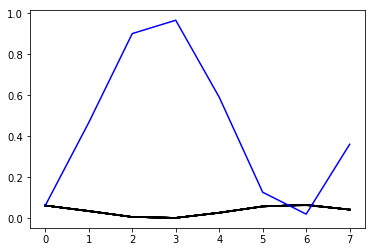
\includegraphics[width=0.99\linewidth]{img/groveralllossless.png}
        \caption{Sin relajación}
    \end{subfigure}
    \begin{subfigure}[m]{0.49\textwidth}
        \centering
        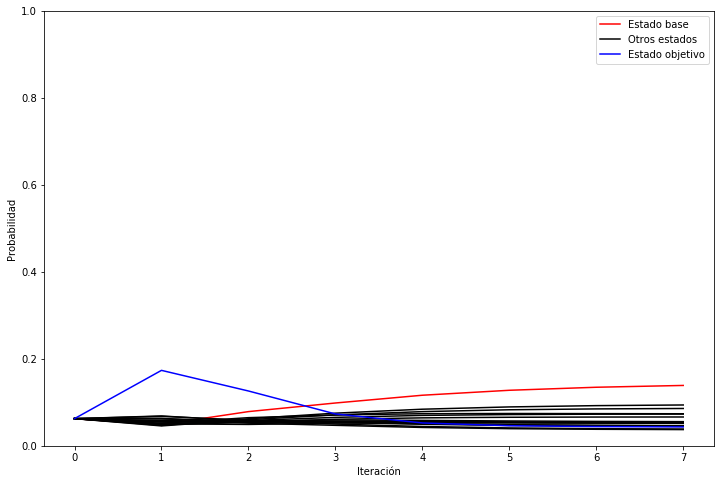
\includegraphics[width=0.99\linewidth]{img/groverallloss.png}
        \caption{Con relajación}
    \end{subfigure}
    \caption[Evolución de las probabilidades en el algoritmo de Grover con relajación]{Evolución de las probabilidades en el algoritmo de Grover con relajación}
    \label{fig:groverlosscomp}
\end{figure}

\subsection{Amplificación de amplitud}

\subsection{Optimización del algoritmo de Grover}

